\section{Modelo de Processo}

Nesta seção é proposto um modelo para a gerência de ordens de serviço. Tal
modelo busca ser aderente às recomendações da IN4, mas busca ao mesmo tempo
possibilitar a customização para as necessidades específicas do órgão que vier
a adotá-lo.

A Figura \ref{fig:so_process} mostra o desenho do processo proposto, sua
sequência e as etapas envolvidas.

\begin{figure}[H]
  \centering
  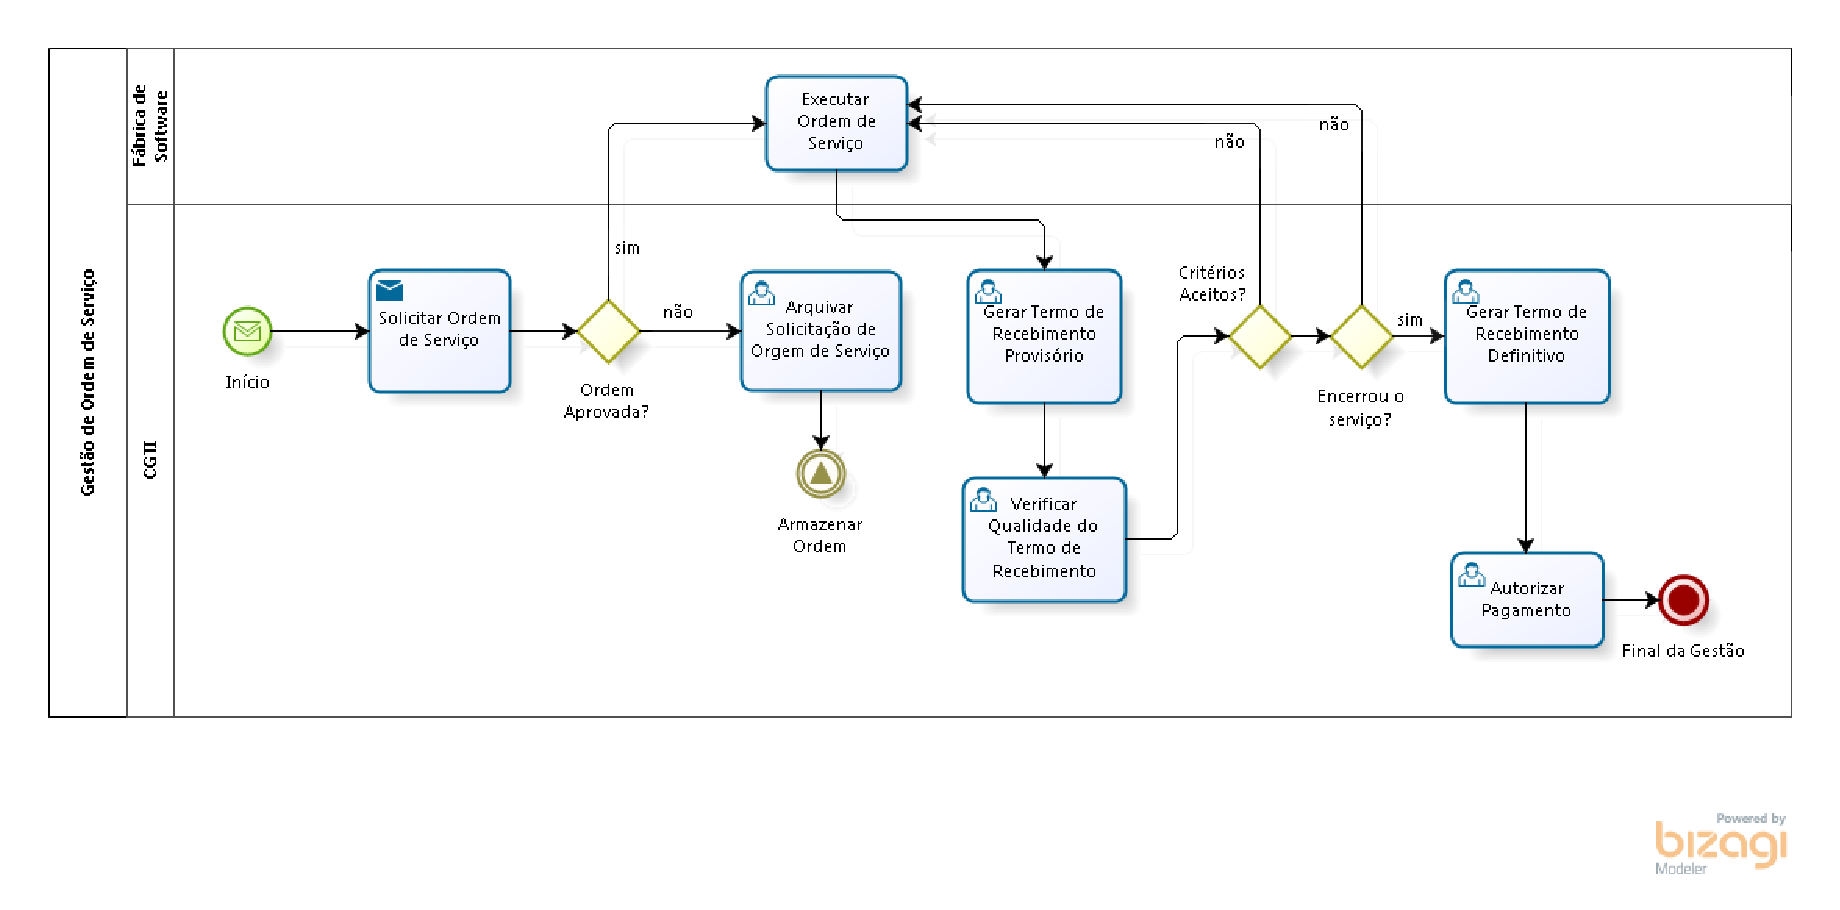
\includegraphics[keepaspectratio=true,scale=0.5]{figures/so_process}
  \caption{Proposta de um processo para gerenciar ordens de serviço.}
  \label{fig:so_process}
\end{figure}

As atividades do processo são descritas a seguir:

\begin{itemize}
  \item \textbf{Solicitar Ordem de Serviço:} realização de uma solicitação de ordem
  de serviço para a requisição de uma nova solução de \textit{software}. A solicitação
  ocorre apartir de uma necessidade já estabelecida;
  \item \textbf{Ordem de Serviço Aprovada?:} verificação de aprovação da ordem de
  serviço quanto ao orçamento e demanda. É possível que esta condicional seja realizada
  por outro processo;
  \item \textbf{Arquivar Solicitação de Ordem de Serviço:} caso a solicitação não seja
  aprovada, a solicitação é arquivada para futuras consultas e insumo para relatórios
  estatísticos;
  \item \textbf{Gerar Termo de Recebimento Provisório:} quando a prestadora
  finaliza o desenvolvimento da ordem de serviço ela deve informar a contratante,
  que deverá, então, gerar o Termo de Recebimento Provisório. Tal termo atesta
  que a prestadora executou o serviço e que partir daquele momento ela aguarda
  a avaliação dos itens desenvolvidos;
  \item \textbf{Verificar Qualidade do Termo de Recebimento:} ao gerar o Termo de Recebimento Provisório,
  a contratante tem a responsabilidade de avaliar o produto desenvolvido, isto é,
  verificar se tudo o que foi desenvolvido está de acordo com o que foi previsto
  na OS. Esta avaliação pode gerar sanções administrativas e devolver a OS para
  execução, caso seja constatado que o serviço não foi executado dentro dos termos.
  No fim, deve-se ter um relatório de qualidade que embase um parecer técnico da
  empresa contratada para avaliar o resultade de outra;
  \item \textbf{Executar Ordem de Serviço:} relacionada inteiramente com a contratada.
  Nesta etapa a contratada irá realizar todos os itens previstos na OS para satisfazer
  as necessidades da contratante;
  \item \textbf{Critérios Aceitos?:} caso os critérios foram aceitaveis, dar-se-a
  continuidade ao processo;
  \item \textbf{Encerrou o Serviço?:} condicional para verificar se todos os itens
  previstos em OS foram realizados. Caso não tenham sido feitos, a condicional volta
  para a execução do serviço;
  \item \textbf{Gerar Termo de Recebimento Definitivo:} se a OS foi corretamente
  executada e os itens entregues correspondem às expectativas descritas na
  OS a contratante deverá então gerar o Termo de Recebimento Definitivo, que
  atesta que a prestadora executou a ordem de serviço e que todos os itens
  acordados na OS foram entregues;
  \item \textbf{Autorizar Pagamento:} por fim, uma vez que o Termo de Recebimento
  definitivo foi emitido é então possível autorizar o departemento especializado para
  a realização do pagamento previsto na OS à prestadora.
\end{itemize}
